% **************************************************
% Document Class Definition
% **************************************************
\documentclass[%
    paper=A4,               % paper size --> A4 is default in Germany
    twoside=true,           % onesite or twoside printing
    openright,              % doublepage cleaning ends up right side
    parskip=full,           % spacing value / method for paragraphs
    chapterprefix=true,     % prefix for chapter marks
    12pt,                   % font size
    headings=normal,        % size of headings
    bibliography=totoc,     % include bib in toc
    listof=totoc,           % include listof entries in toc
    titlepage=on,           % own page for each title page
    captions=tableabove,    % display table captions above the float env
    draft=false            % value for draft version
]{scrreprt}%


% **************************************************
% Setup YOUR thesis document in this file !
% **************************************************
% !TEX root = thesis.tex


% **************************************************
% Files' Character Encoding
% **************************************************
\PassOptionsToPackage{utf8}{inputenc}
\usepackage{inputenc}


% **************************************************
% Information and Commands for Reuse
% **************************************************
\newcommand{\thesisTitle}{One-shot recognition for art historic images}
\newcommand{\thesisName}{Maurice Frank}
\newcommand{\thesisSubject}{Documentation}
\newcommand{\thesisDate}{May 17, 2017}
\newcommand{\thesisVersion}{v1.0}

\newcommand{\thesisFirstReviewer}{Björn Ommer}
\newcommand{\thesisFirstReviewerUniversity}{\protect{University of Heidelberg}}
\newcommand{\thesisFirstReviewerDepartment}{Department of Mathematics and Computer Science}

\newcommand{\thesisSecondReviewer}{John Doe}
\newcommand{\thesisSecondReviewerUniversity}{\protect{University of Heidelberg}}
\newcommand{\thesisSecondReviewerDepartment}{Department of Mathematics and Computer Science}

\newcommand{\thesisFirstSupervisor}{Miguel Angel Bautista}

\newcommand{\thesisUniversity}{\protect{University of Heidelberg}}
\newcommand{\thesisUniversityDepartment}{Department of Mathematics and Computer Science}
\newcommand{\thesisUniversityInstitute}{Heidelberg Collaboratory for Image Processing}
\newcommand{\thesisUniversityGroup}{Computer Vision Research Group}
\newcommand{\thesisUniversityCity}{Heidelberg}
\newcommand{\thesisUniversityStreetAddress}{Berliner Str. 43}
\newcommand{\thesisUniversityPostalCode}{69120}


% **************************************************
% Debug LaTeX Information
% **************************************************
%\listfiles


% **************************************************
% Load and Configure Packages
% **************************************************
\usepackage[english]{babel} % babel system, adjust the language of the content
\PassOptionsToPackage{% setup clean thesis style
    figuresep=colon,%
    sansserif=false,%
    hangfigurecaption=false,%
    hangsection=true,%
    hangsubsection=true,%
    colorize=full,%
    colortheme=redyellow,%
    bibsys=biber,%
    bibfile=assets/references,%
    bibstyle=alphabetic,%
    wrapfooter=false,%
}{cleanthesis}
\usepackage{cleanthesis}

\hypersetup{% setup the hyperref-package options
    pdftitle={\thesisTitle},    %   - title (PDF meta)
    pdfsubject={\thesisSubject},%   - subject (PDF meta)
    pdfauthor={\thesisName},    %   - author (PDF meta)
    plainpages=false,           %   -
    colorlinks=false,           %   - colorize links?
    pdfborder={0 0 0},          %   -
    breaklinks=true,            %   - allow line break inside links
    bookmarksnumbered=true,     %
    bookmarksopen=true          %
}

\usepackage[xindy, toc]{glossaries}
\makeglossaries
\newacronym{fcn}{FCN}{Fully Convolutional Network}


\usepackage{tikz}
\usetikzlibrary{arrows,chains,matrix,positioning,scopes}

\newcommand{\bigO}[1]{$\mathcal{O}(#1)$}


\usepackage{multirow}



% **************************************************
% Document CONTENT
% **************************************************
\begin{document}

% --------------------------
% rename document parts
% --------------------------
%\renewcaptionname{ngerman}{\figurename}{Abb.}
%\renewcaptionname{ngerman}{\tablename}{Tab.}
\renewcaptionname{english}{\figurename}{Fig.}
\renewcaptionname{english}{\tablename}{Tab.}

% --------------------------
% Front matter
% --------------------------
\pagenumbering{roman}			% roman page numbing (invisible for empty page style)
\pagestyle{empty}				% no header or footers
% !TEX root = ../thesis.tex
%
% ------------------------------------  --> cover title page
\begin{titlepage}
	\pdfbookmark[0]{Cover}{Cover}
	\flushright
	\hfill
	\vfill
	{\Large\thesisTitleGerman \par}
	{\LARGE\thesisTitle \par}
	\rule[5pt]{\textwidth}{.4pt} \par
	{\Large\thesisName}
	\vfill
	\textit{\large\thesisDate} \\
\end{titlepage}


% ------------------------------------  --> main title page
\begin{titlepage}
	\pdfbookmark[0]{Titlepage}{Titlepage}
	\tgherosfont
	\centering

	{\Large \thesisUniversity} \\[4mm]
	\textsf{\thesisUniversityDepartment} \\
	\textsf{\thesisUniversityInstitute} \\
	\textsf{\thesisUniversityGroup} \\

	\vfill
	{\large \thesisSubject} \\[5mm]
	{\Large \color{ctcolortitle}\textbf{\thesisTitleGerman} \\[10mm]}
	{\LARGE \color{ctcolortitle}\textbf{\thesisTitle} \\[10mm]}
	{\Large \thesisName} \\
	{\large \thesisStudentID} \\

	\vfill
	\begin{minipage}[t]{.27\textwidth}
		\raggedleft
		\textit{Reviewer}
	\end{minipage}
	\hspace*{15pt}
	\begin{minipage}[t]{.65\textwidth}
		{\Large \thesisFirstReviewer} \\
	  	{\small \thesisFirstReviewerDepartment} \\[-1mm]
		{\small \thesisFirstReviewerUniversity}
	\end{minipage} \\[5mm]
	% \begin{minipage}[t]{.27\textwidth}
	% 	\raggedleft
	% 	\textit{2. Reviewer}
	% \end{minipage}
	% \hspace*{15pt}
	% \begin{minipage}[t]{.65\textwidth}
	% 	{\Large \thesisSecondReviewer} \\
	%   	{\small \thesisSecondReviewerDepartment} \\[-1mm]
	% 	{\small \thesisSecondReviewerUniversity}
	% \end{minipage} \\[10mm]
	\begin{minipage}[t]{.27\textwidth}
		\raggedleft
		\textit{Supervisors}
	\end{minipage}
	\hspace*{15pt}
	\begin{minipage}[t]{.65\textwidth}
		\thesisFirstSupervisor
	\end{minipage} \\[10mm]

	\thesisDate \\

\end{titlepage}


% ------------------------------------  --> lower title back for single page layout
\hfill
\vfill
{
	\small
	\textbf{\thesisName} \\
	\textit{\thesisTitle} \\
	\textit{\thesisTitleGerman} \\
	\thesisSubject, \thesisDate \\
	Reviewers: \thesisFirstReviewer\\ %\ and \thesisSecondReviewer \\
	Supervisors: \thesisFirstSupervisor \\[1.5em]
	\textbf{\thesisUniversity} \\
	\textit{\thesisUniversityGroup} \\
	\thesisUniversityInstitute \\
	\thesisUniversityDepartment \\
	\thesisUniversityStreetAddress \\
	\thesisUniversityPostalCode\ and \thesisUniversityCity
}
		% INCLUDE: all titlepages
\cleardoublepage

\pagestyle{plain}				% display just page numbers
% !TEX root = ../thesis.tex
%
\pdfbookmark[0]{Abstract}{Abstract}
\chapter*{Abstract}
\label{sec:abstract}
\vspace*{-15mm}
This thesis introduces a one-shot object detector that was developed with the objective to retrieve similar objects from images given a single reference object. We show that using a, for image classification pretrained, neural network, it is possible to train a object detector from small numbers of examples in very little time. Our results show the connection and correllation between the number of examples and the quality of the detector. Furthermore we show how, using intensive preprocessing, a single example can be enough to extract similar instances.\TODO{finish}

\vspace*{20mm}

{\usekomafont{chapter}Zusammenfassung}\label{sec:abstract-diff} \vspace*{5mm}\\
Diese Abschlussarbeit führt einen Objektdetektor ein, der mit dem Ziel entwickelt wurde ähnliche Objekte in Bildern zu finden mit einer einzelnen vorgegebenen Referenz. Wir zeigen, dass es unter der Verwendung eines für Bildklassifikation trainierten Neuronalen Netzwerks möglich ist, einen Detekor auf Basis weniger Beispiele in kürzester Zeit zu trainiern. Unsere Resultate verdeutlichen den Zusammenhang, zwischen der Anzahl der verschiedenen Beispiele und der Qualität des Detektors. Weiterhin wird gezeigt, wie mit umfangreicher Vorverarbeitung der Referenz, schon ein einzelnes Bild reichen kann, um ähnliche Instanzen zu finden.
		% INCLUDE: the abstracts (english and german)
\cleardoublepage
%
\setcounter{tocdepth}{2}		% define depth of toc
\tableofcontents				% display table of contents
\cleardoublepage

% --------------------------
% Body matter
% --------------------------
\pagenumbering{arabic}			% arabic page numbering
\setcounter{page}{1}			% set page counter
\pagestyle{maincontentstyle} 	% fancy header and footer

% !TEX root = ../thesis.tex
%
\chapter{Introduction}
\label{sec:intro}

\section{Motivation and Problem Statement}
\label{sec:intro:motivation}

\section{Results}
\label{sec:intro:results}

\section{Thesis Structure}
\label{sec:intro:structure}

\textbf{Chapter \ref{sec:concepts}} \\[0.2em]
   % INCLUDE: introduction
% % !TEX root = ../thesis.tex
%
\chapter{Related Work}
\label{sec:related}
In this chapter we quickly want to revise other works touching the the tasks of this thesis. In \treft{sec:related:detection} we discuss multiple successful object detection methods using \glspl{cnn}. In \treft{sec:related:oneshot} we describe two solutions to the task of one-shot learning and lastly in \treft{sec:related:retrieval} we list examples of the application of such detection systems as image search systems.

\section{Object detection}
\label{sec:related:detection}
The first work to approach object detection with \glspl{cnn} where \citet{girshick_rich_2014} with their \textbf{\gls{rcnn}}. For each image they use Selective Search to generate a set of region proposals. Selective Search is a technique to identify possible object-like but type independent regions probing texture and color on multiple scales. All these boxes are reshaped to a uniform size and forwarded through a normal classification network (in their case AlexNet) to yield feature vectors from the \gls{fc} layers for each box. Lastly a multi-class \gls{svm} classifies these proposols. Additionally the \gls{rcnn} is trailed by a linear regression model which uses the classified boxes to produce tighter box coordinates. Although the results proved that \glspl{cnn} can greatly improve detection results the method is rather hard to train as classifier network, \gls{svm} and regressor have to be trained independently and moreover classifying each region box independently is extremely slow.

A year later again \citet{girshick_fast_2015} released \textbf{Fast \gls{rcnn}} which improves computation performance and training complexity. Instead of computing features for each proposed region Fast \gls{rcnn} computes the features for the whole image once. Then the regions in the image are projected onto the feature map of the network thus yielding the patch-wise features. Then those are pooled and put through \gls{fc} layers and finally into a classifier and the box regressor. The \gls{svm} is replaced with a SoftMax and the linear regression model with a additional \gls{fc} layer. As such the three models from \gls{rcnn} become one which is are end-to-end trainable.

In the same year \citet{ren_faster_2015} tackled the last bottleneck of this approach which is the region proposal system with their \textbf{Faster \gls{rcnn}}. The previously used Selective Search is rather slow and still independent of the model. Using also the features generated by the \gls{conv} layers they add a new network branch, a \gls{rpn}, to generate boxes that are used for the same \gls{roi} pooling as in the Fast \gls{rcnn}. The \gls{rpn} is a \gls{fcn} that slides over the feature map and at each positions tests for a predefined set of $k$ anchor boxes whether those could be objects. So for each window the \gls{rpn} outputs a score of \textit{objectness} and coordinates of the bounding box. Those are then the inputs for the Fast \gls{rcnn} method.

Two year late \citet{he_mask_2017} extended this approach with \textbf{Mask \gls{rcnn}} to pixel-wise segmentation of images. In the previous versions the regions from the original image were projected onto the feature maps by just down-scaling their shapes with the respective factor and discretizing them on the feature grid. This rounding introduces errors in the proposed bounding boxes and leads to misalignment. Instead they use bilinear interpolation inside each region to find more precise feature representations. This process is done by a new network branch inside the Faster \gls{rcnn} and outputs binary pixel-wise masks for each \gls{roi}. The regions are classified as in the Faster \gls{rcnn} and generate therefore semantic image segmentations.

\citet{dai_r-fcn:_2016} incorporates the \gls{roi}-wise processing into the main network branch of their \textbf{R-FCN} through a series of \gls{conv} layers. The \gls{conv} layers encode scores at relative positions like top-left or bottom-center. Next the regions from the \gls{rpn} are divided into the same relative sub-regions and each sub-region is used to pool from the corresponding layer and then vote for the whole \gls{roi}.

As out work also has to focus on time performance it is related to other fast object detectors. \citet{redmon_you_2016} use a freshly designed network architecture \textbf{YOLO} to achieve object detection at real-time. The input image is divided into a regular grid. The last \gls{fc} layer from their network predicts for each cell of the grid the class probabilities and the coordinates and objectness confidence of two bounding boxes. Detections then get selected by the multiplication of their conventional class probabilities and their individual confidence predictions. While the method is extremely fast it is limited by the shape of bounding boxes it will predict.

\section{Similarity retrieval}
\label{sec:related:retrieval}
\begin{my_list}
    \item \citet{wang_learning_2014}
    \item \citet{chen_visual-based_2015}
\end{my_list}
   % INCLUDE: related work
% % !TEX root = ../thesis.tex
%
\chapter{Pipeline}
\label{sec:pipeline}

\section{Generating detections}
\label{sec:pipeline:eval}
Our desired output of the algorithm is one or are multiple boxes enclosing each a section of the image which is predicted to contain the searched for type of object. The \gls{fcn} returns a score map as output. Each score predicts the probability of this pixel to be of the class we trained for. Therefore we need a method to return high scoring bounding boxes from a probability map. The here employed way of doing this consists of multiple steps:\\
\begin{enumerate}
    \item We penalize (near-) empty regions inside the probability map with a negative distance transform
    \item We generate a set of beforehand defined boxes
    \item For all these boxes we calculate the score density
    \item We apply a low threshold to filter out unnecessary boxes
    \item We apply non maximum suppression to get the top scoring boxes
\end{enumerate}

\subsection{Negative Distance Transform}
\label{sec:pipeline:eval:dt}
\begin{figure}[htb]
    \begin{tabular}{ccc}
        
\includegraphics[width=45mm]{figures/build/distance_transform_hm} &
        
\includegraphics[width=45mm]{figures/build/distance_transform_thres} &
        
\includegraphics[width=45mm]{figures/build/distance_transform_negative} \\[6pt]
        (a) A probability map & (b) Thresholded map & (c) Distance transform
    \end{tabular}
	\caption{Computing the negative distance transform from an probability map}
    \label{fig:distance_transform}
\end{figure}
A lot of images produce probability maps that are sparsely filled. We want to penalize these regions. Positive regions receive a positive score from the network while not-positive regions are at-most zero. Here we introduce a distance transform to score regions of near-zero values \fref{fig:distance_transform}. First we threshold the score map with a near-zero value to set all values that can safely assumed to be negatives to zero. Second we apply a distance transform to the zero part of the binary image. A distance transform labels each zero pixel of an image with its distance to the nearest one valued pixel. The distances are valued with some metric like the Euclidean distance or the $L_1$ distance. As the specific metric is not important for our vague penalizer and as we aim for good time performance we use the $L_\infty$ distance also known as the chessboard distance. The transformed image is normalized and substracted from the original probability map.

\subsection{Calculating the score densities}
\label{sec:pipeline:eval:density}
For each forwarded image we generate a set of boxes to calculate the score densities for. At three scales we take boxes of the same aspect ratio as the input image and calculate the slices that would be the result of sliding the window over the image. Also we save the area of all rectangles.\\
Density is calculated by summing up all the probabilities from the score map inside the current window and dividing this sum by the area of the window. To achieve that as efficiently as possible we use the integral image of our score map. By summing up all values from the top-left corner to the bottom-right corner of an image we get its integral. A value of the integral then is the sum of all values inside the rectangle of this point and the top-left corner:
\begin{equation}
    I_{int}(x, y) = \sum_{\substack{x' \le x\\ y' \le y}} I(x', y')
\end{equation}
The sum inside any rectangle can then computed efficiently with:
\begin{equation}
    \sum_{\substack{x_0 < x \le x_1\\ y_0 < y \le y_1}} = I_{int}(x_1, y_1) + I_{int}(x_0, y_0) - I_{int}(x_1, y_0) - I_{int}(x_0, y_1)
\end{equation}

\subsection{Non maximum suppression}
\label{sec:pipeline:eval:nms}
Depending on the number of scales we generate hundreds or even thousands of boxes per image. We want to eliminate boxes that are overlapping with another box that has a higher density. Firstly we drop the worst boxes with a low set threshold. To the remaining boxes we apply non maximum suppression as described by \citet{felzenszwalb_discriminatively_2008}. In the non maximum suppression we first sort all boxes by their descending scores which in our case are the probability densities. We mark the strongest box as picked. Then we calculate the area overlap between the new picked box and all remaining boxes. All boxes with an overlap in area of 0.5 or more are dropped. We pick the next strongest score of the remaining set and continue this process until all boxes are either dropped or picked. The strongest not-overlapping boxes remain picked and are returned.
         % INCLUDE: system
% !TEX root = ../thesis.tex
%
\chapter{Concepts}
\label{sec:concepts}

\cleanchapterquote{Q: What's the difference between machine learning and statistics?\\A: ConvNets}{Bored Yann LeCun}{via Twitter}

\section{Machine learning}
\label{sec:concepts:ml}

\section{Task definitions}
\label{sec:concepts:tasks}
Although the posed task for this thesis is pretty clear from its formulation we want to quickly distinguish the similar but different image understanding tasks that are solved using these techniques.

The first task that was tackled is \textbf{image classification}. In image classification the data are images containing a single object that fills most of the image. Hence the task is to find the class of that singular object which thus describes the whole image. Since 2015 \glspl{cnn} can surpass the performance of humans doing classification \citep{he_delving_2015}.

Next \textbf{object localization} was addressed. Localization means that we still have only one relevant object per image but here the object fills only a part of the image. Instead of only predicting the class of this object the localizer also has to predict translation and scaling for each image.

Harder to solve but also way more applicable is \textbf{object detection}. Now we take complicated images containing a variable number of overlapping objects each of varying class. The detector identifies all objects he was trained for inside each image and predicts their boundaries.

Lastly we have \textbf{image segmentation}. Here we aim to not only identify multiple different object in a image but also to find their boundaries on the pixel level. As such each pixel of a found object in the image is labeled with its class id resulting in multiple binary masks each masking out one individual object.

\section{Neural Networks}
\label{sec:concepts:nn}

\subsection{Convolutions} % (fold)
\label{sub:conepts:nn:conv}

\subsection{Activation Functions} % (fold)
\label{sub:conepts:nn:activations}
\begin{figure}
    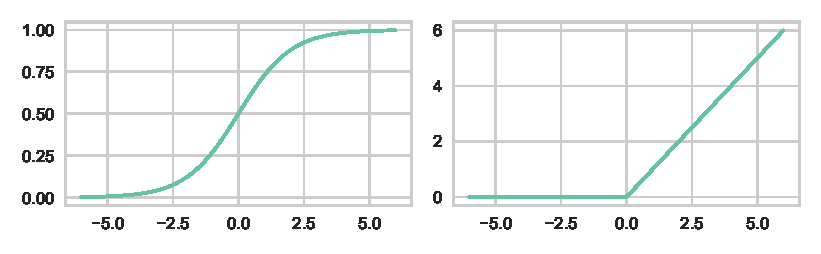
\includegraphics{figures/build/sigmoid_relu}
    \caption{Activation functions: sigmoid on the left and \gls{relu} on the right.}
    \label{fig:sigmoid_relu}
\end{figure}
\begin{figure}
    \centering
    \begin{tabulary}{\linewidth}{CCCC}
        
\includegraphics[height=3cm]{figures/build/activation_data} &
        \vspace{-1.8cm}\includegraphics[height=1cm]{figures/build/activation_filter-img0} &
        \includegraphics[height=3cm]{figures/build/activation_response-img0} &
        \includegraphics[height=3cm]{figures/build/activation_relu-img0} \\
        image data & filter & filter response & \gls{relu} \\
    \end{tabulary}
    \caption{The effect of \gls{relu} visualized. The green activations are positive and the purple ones are negative.}
\end{figure}
\gls{conv} layers return the response of their inputs to their filters. Next the response level is used to calculate how much the node fires for this position in the receptive field. Conceptually this draws from the activation process inside neurons in the brain which also receive inputs from their dendrites and fire along their axon. Inside a artificial neural network this mapping is done by an activation function $f(x)$. In the most simple cases this can be the identity $f(x) = x$ or the unit step function $f(x) = (\sign x + 1) / 2$. With the identity we just use the response values as firing rates not introducing any more complexity and the sign reduces the levels of response to a binary firing switch.

Formerly common to use was the sigmoid as an activation function. The sigmoid $\sigma(x) = 1/(1+e^{-x})$ \fref{fig:sigmoid_relu} takes an unbounded input range and squashes it into the range $[0, 1]$. Today sigmoids are mostly avoided as they hold multiple drawbacks. First as the sigmoid saturates in both directions its gradient can approximate zero which with backpropagation will result in a generally zeroed gradient. Secondly is the gradient computation slowed due to the non-linear form.

As shown before convolutions are linear operations. A chain of convolutions would still return a linear classifier but we know that working on raw pixel values from our images it will in the most cases be impossible to linearly separate the different classes \citep{lecun_deep_2015}. To discriminate such representation we need a non-linear division boundary and thus a \gls{cnn} should be a composite of linear and non-linear operations so that at least in theory it can approximate the non-linear representation. Therefore a non-linear activation function is important in most network architectures.

One popular function to hold those properties is the rectifier $\rho(x) = max(0, x)$ \fref{fig:sigmoid_relu} employed in \glspl{relu}. While being piecewise linear and therefore computationally efficient the rectifier is a non-linear function. As it is saturating it avoids the problems of zeroed or exploding gradients that the sigmoid has.

\subsection{Pooling}
\label{sub:concepts:nn:pooling}
A typical building block for \glspl{cnn} is the triple of a \gls{conv} layer followed by a non-linear activation function followed by a pooling layer. The pooling layer takes its input from the previous layer and compresses spatially into into a smaller form. Different function can be applied to the data neighborhood from the input. Average pooling \citep{lecun_handwritten_1990} or max pooling \citep{zhou_computation_1988} are two of the most prominent ones. With average pooling we return the average of the values from the neighborhood and with max pooling we return the maximum value from the neighborhood.

It is important to note that average pooling is a linear function while max pooling is not. \glspl{cnn} should compose a non-linear function. Thus pooling is can be used to introduce non-linearity and therefore max pooling is more popular to use. Also as downsampling of the deep filters can be done with strided convolutions alone pooling is not necessary for this and more and more network architectures drop the pooling layers entirely \citep{springenberg_striving_2014}.

\subsection{Regularization} % (fold)
\label{sub:conepts:nn:regularization}

\subsection{Batch Normalization} % (fold)
\label{sub:conepts:nn:batchnorm}
Batch normalization \citep{ioffe_batch_2015} is a method the ease the computation of gradient descent in backpropagation and also to reduce problems of bad weight initialization. Inside a deep neural network emerges the problem of internal covariate shift. Each deeper layer of the network depends on the outputs from its previous layer. The first layer learns on top of the data input but the second layer learns from the output of the first layers features and the third layer depends on the second one and so on. In training all these features change through backpropagation and the distribution of all activations change and the deeper the layer is the longer the chain of evolving distributions in front of it becomes.\\
If the features in training shift over time the gradient decent becomes harder as each layer has to follow this covariate shift of its successor. BatchNorm helps to avoid this difficulty by normalizing mini batches of inputs. The layer is added after a convolutional layer (or any other linear layer) and collects a batch of inputs $X = \{x_1, x_2, x_3, \dots, x_n\}$ for this layers inputs. Then it calculates the mean $\mu_X$ and the variance $\sigma_X^2$ for this mini batch. Normalizing all the values from that batch  with
\begin{equation}
    \hat{x_i} = \frac{x_i - \mu_X}{\sqrt{\sigma_X^2 + \epsilon}}
\end{equation}
($\epsilon$ is added to avoid divisions by zero) yields the output $\{\hat{x_1},\dots,\hat{x_n}\}$.\\
To use the BatchNorm parameters while testing we compute a moving average over the means and variances of the batches while training. The forward pass uses these averages to normalize the test inputs.

\section{Fully Convolutional Networks}
\label{sec:concepts:fcn}
Proposed by \citet{long_fully_2015} \glspl{fcn} are a specific architecture of \glspl{cnn}. Fully convolutional states that the network consists only of convolutional layers. As these are translation invariant the networks can take arbitrarily sized inputs and produce a coarse output.

The original authors use this architecture for image segmentation. They build their network from classic semantic object classifiers like VGG-16 \citep{simonyan_very_2014}. These take fixed sized images as inputs and produce a single label thereby classifying the whole image. Typically these networks produce high level features through a series of convolutional layers and classify them with a single or a series of \gls{fc} layers. To label an image pixel-wise with such an architecture we would have to forward the neighborhood of each pixel through the network which would introduce an \bigO{w * h} time complexity ($w$ and $h$ being the width and the height of the image).

\subsection{Deconvolution} % (fold)
\label{sub:conepts:fcn:deconv}

\begin{figure}[h]
    \centering
    \begin{tabular}{cc}
    \begin{tikzpicture}[font=\footnotesize\sffamily]
        \fill[black!20] (1,3) rectangle (2,3.5);
        \fill[black!20] (6,3) rectangle (7,3.5);

        \foreach \x/\y in {1/2, 2/1.5, 3/1, 4/0.5, 5/0}
            \fill[set2_1!50] (\x, \y) rectangle (\x + 2, \y + 0.5);

        \fill[black!20] (1,2) rectangle (2,2.5);
        \fill[black!20] (6,0) rectangle (7,0.5);

        \foreach \x/\y in {1/2, 2/1.5, 3/1, 4/0.5, 5/0}
        {
            \node[above right] at (\x + 0.0, \y) {1};
            \node[above right] at (\x + 0.5, \y) {2};
            \node[above right] at (\x + 1.0, \y) {3};
            \node[above right] at (\x + 1.5, \y) {4};
        }

        \draw[step=0.5cm,gray,very thin] (0,0) grid (0.5,2.5);
        \draw[step=0.5cm,gray,very thin] (0.99,2.99) grid (7,3.5);
        \draw[step=0.5cm,gray,very thin] (0.99,0) grid (7,2.5);
        \draw [->] (2.25,3.25) -- (2.25,2);
        \draw [->] (2.75,3.25) -- (2.75,2);
        \draw [->] (3.25,3.25) -- (3.25,2);
        \draw [->] (3.75,3.25) -- (3.75,2);
        \draw [->] (1.9,1.75) -- (0.5,1.75);
    \end{tikzpicture} &
    \begin{tikzpicture}[font=\footnotesize\sffamily]
        \fill[black!20] (0,5) rectangle (0.5,6);
        \fill[black!20] (0,0) rectangle (0.5,1);

        \foreach \y/\x in {4/1, 3/1.5, 2/2, 1/2.5, 0/3}
            \fill[set2_1!50] (\x, \y) rectangle (\x + 0.5, \y + 2);

        \fill[black!20] (1,5) rectangle (1.5,6);
        \fill[black!20] (3,0) rectangle (3.5,1);

        \foreach \y/\x in {4/1, 3/1.5, 2/2, 1/2.5, 0/3}
        {
            \node[above right] at (\x, \y + 1.5) {1};
            \node[above right] at (\x, \y + 1.0) {2};
            \node[above right] at (\x, \y + 0.5) {3};
            \node[above right] at (\x, \y) {4};
        }

        \draw[step=0.5cm,gray,very thin] (0.99,6.49) grid (3.5,7);
        \draw[step=0.5cm,gray,very thin] (0,0) grid (0.5,6);
        \draw[step=0.5cm,gray,very thin] (0.99,0) grid (3.5,6);
        \draw [->] (1.25,6.75) -- (1.25,5);
        \draw [->] (1.75,6.75) -- (1.75,5);
        \draw [->] (1,4.75) -- (0.5,4.75);
        \draw [->] (1,4.25) -- (0.5,4.25);
    \end{tikzpicture} \\[6pt]
    (a) Convolution & (b) Transposed Convolution
    \end{tabular}
    \caption{Convolution with stride 2 in 1D and transposed convolution with stride 2. Input signals are at the top, output is to the right and the gray boxes are padding. With the arrows we note how input points contribute to the output. The convolution applies a filter of size 4 to an signal of size 8 and with the padding produces an output of size 5. The transposed convolution in return takes a input of 5 and returns a signal of size 10. Figure is based on \citep{shi_is_2016}.}
    \label{fig:1d_strided_conv}
\end{figure}

Deconvolution or often called transposed convolution, first used by \citet{zeiler_deconvolutional_2010}, introduces a new operation for neural networks. Simply spoken a deconvolution takes the receptive field and produces a larger window as output thus operating some form of upsampling. \figreft{fig:1d_strided_conv} visualizes the differences between convolution and deconvolution in $1-d$.

\subsection{Conversion of \gls{fc} layers}
\label{sub:concepts:fcn:fc_conversion}
\gls{fc} layers can directly be converted into \gls{conv} layers which makes \glspl{fcn} immensely efficient.\\
To understand this process let us examine the VGG-16 network. After the 13 \gls{conv} layers and 5 max-pooling layers we get an output from \texttt{pool5} with size $512\times7\times7$. Through pooling the original images ($224\times224$) got reduced to $7\times7$ images over 512 channels. These go though 3 \gls{fc} layers. The first \gls{fc} layer returns 4096 values. We replace it with a \gls{conv} layer with kernel size 7 and 4096 channels thus resulting also in $1\times1\times4096$ output volume. The weights from the \gls{fc} layer can be reshaped into the size of the \gls{conv} layer. The other two \gls{fc} layers with 4096 and 1000 outputs, respectively can directly be put into convolutions with kernel size 1.

For the normal $224\times224$ images nothing changed as the output of the first \gls{fc} layer is still the 4096 values but if we now increase the data size to e.g. the double $448\times448$ the advantage becomes apparent. The \texttt{pool5} will return $14\times14$ images and the new \gls{conv} layer will just slide over the bigger images returning $8\times8$ images. Lastly the other $1\times1$ convolutions do not change the size so that we get 64 predictions over the 1000 classes instead of one. These are the same as if we would have slided a window over the original image with an $8\times8$ grid but because the computations on the GPU are shared for the $7\times7$ kernels we heavily increased performance compared to the naïve solution.

\subsection{Upsampling through Convolutions}
\label{sub:concepts:fcn:upsampling}
A \gls{fcn} as in \citep{long_fully_2015} outputs a small sparse score map. For an input image of $200\times 200$ pixels that could be something like $10\times 10$ values. Naturally we want a output map with the same size as the input. Firstly we can use feature maps from earlier layers with their own classifiers to reduce the stride of the resulting score map but the score map from deeper layers has still to be upsampled to the input size. Upsampling can be done directly within the network with convolutions. It is possible to use deconvolutions to upsample the inputs and filter them at the same time but this often introduces artifacts \citep{odena_deconvolution_2016} and to learn the upsampling instead of using directly bilinear kernels does not help much in performance \citep{shelhamer_fully_2016}. It seems successful to upsample the score maps with normal interpolation followed by normal convolutions \citep{dong_image_2016}.

\section{Residual Networks}
\label{sec:concepts:resnet}
After the succes of AlexNet \citep{krizhevsky_imagenet_2012} and with the possibilities of fast GPU computing neural networks got deeper and bigger.
The VGG-16 by \citet{simonyan_very_2014} has 442.5 million trainable parameters for its 16 layers. The more parameters a network has the harder the training becomes.
Since the last years multiple new network architectures were developed that achieve higher accuracy with less parameters and therefore shorter inference time \citep{canziani_analysis_2016}. One of those architectures are \gls{resnet} by \citet{he_deep_2016} with which they won the COCO  \citet{lin_microsoft_2014} and the ImageNet \citet{russakovsky_imagenet_2015} object detection challenges in 2015.
A \gls{conv} layer in a standard feed forward network learns a mapping $\mathcal{H}(x)$ from its input $x$. When training the network we reach the point at which the accuracy saturates. At this point the layers which are further trained should approximate a identity mapping of their inputs as the optimum has already been reached. In practice with deep networks new layers at some point in training rapidly mode away from the identity they should learn and degrade the training error after it already saturated. Thus making these networks deeper will worsen their results \citep{he_convolutional_2015}.
\begin{figure}
    \centering
    \begin{tabular}{p{6cm}p{6cm}}
    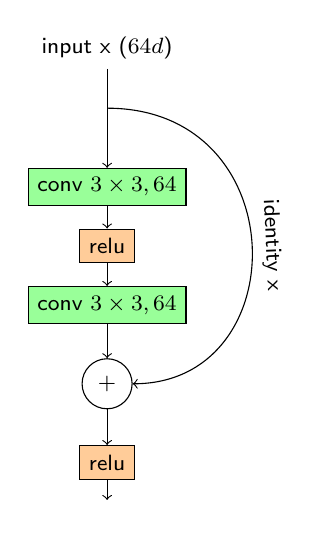
\begin{tikzpicture}[font=\footnotesize\sffamily]
        \path (0, 5) node[above](xinp) {input x ($64d$)}
              (0, 3.5) node[fill=green!40, draw](xc1) {\gls{conv} $3\times3, 64$}
              (0, 2.75) node[fill=orange!40, draw](xr1) {\gls{relu}}
              (0, 2) node[fill=green!40, draw](xc2) {\gls{conv} $3\times3, 64$}
              (0, 1) node[circle,draw](xplus) {+}
              (0, 0) node[fill=orange!40, draw](xend) {\gls{relu}}
              (0, -0.6) node(xout) {};
        \draw[->] (xinp) -- (xc1);
        \draw[->] (xc1) -- (xr1);
        \draw[->] (xr1) -- (xc2);
        \draw[->] (0, 4.5) .. controls +(right:2.4cm) and +(right:2.4cm) .. node[sloped, above] {identity x} (xplus);
        \draw[->] (xc2) -- (xplus);
        \draw[->] (xplus) -- (xend);
        \draw[->] (xend) -- (xout);
    \end{tikzpicture} &

    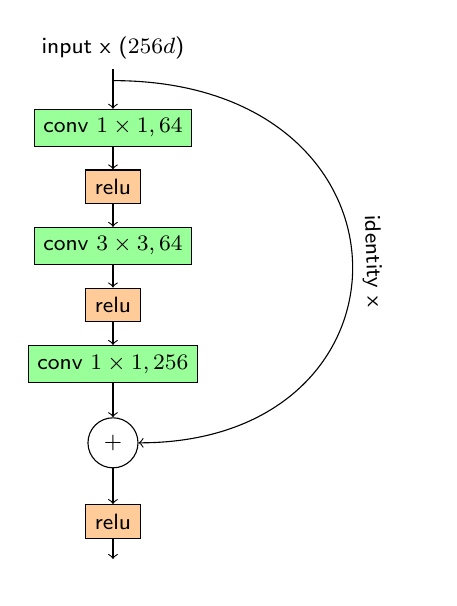
\begin{tikzpicture}[font=\footnotesize\sffamily]
        \path (0, 5.75) node[above](xinp) {input x ($256d$)}
              (0, 5) node[fill=green!40, draw](xc1) {\gls{conv} $1\times1, 64$}
              (0, 4.25) node[fill=orange!40, draw](xr1) {\gls{relu}}
              (0, 3.5) node[fill=green!40, draw](xc2) {\gls{conv} $3\times3, 64$}
              (0, 2.75) node[fill=orange!40, draw](xr2) {\gls{relu}}
              (0, 2) node[fill=green!40, draw](xc3) {\gls{conv} $1\times1, 256$}
              (0, 1) node[circle,draw](xplus) {+}
              (0, 0) node[fill=orange!40, draw](xend) {\gls{relu}}
              (0, -0.6) node(xout) {};
        \draw[->] (xinp) -- (xc1);
        \draw[->] (xc1) -- (xr1);
        \draw[->] (xr1) -- (xc2);
        \draw[->] (xc2) -- (xr2);
        \draw[->] (xr2) -- (xc3);
        \draw[->] (0, 5.6) .. controls +(right:4cm) and +(right:4cm) .. node[sloped, above] {identity x} (xplus);
        \draw[->] (xc3) -- (xplus);
        \draw[->] (xplus) -- (xend);
        \draw[->] (xend) -- (xout);
    \end{tikzpicture}
    \\[6pt]
    (a) A simple non-linear residual block. & (b) A bottleneck block as employed in the deeper \glspl{resnet}.
    \end{tabular}

    \caption{Two examples of residual blocks. The input of the block is fused into the ouptut of the last \gls{conv} layer and added element-wise channel-per-channel onto it. A \gls{relu} is trailing the sum again.}
    \label{fig:resblock}
\end{figure}


The main idea of \glspl{resnet} is pretty simple. They are build from many small identical blocks of which one example is shown in \figreft{fig:resblock}. Instead of blocks that learn the mapping $\mathcal{H}(x)$ we introduce blocks that learn the \textit{residual} $\mathcal{F}(x) = \mathcal{H}(x) - x$ of this mapping. For that we add skip connections between the input and the output of these blocks so that the input can be added to the residual that is the output of the \gls{conv} layers. Learning the residual instead of the actually mapping has the advantage that if new \gls{conv} layers are added and stay unlearned the whole residual block still yields the identity mapping which will not lead to the degradation problem we see with normal deep networks.

\subsection{Network design}
\label{sec:concepts:resnet:design}
Using the basic concept of residual blocks we build a successful architecture. First lets look at what the blocks can contain. The first example in \figreft{fig:resblock} uses just two \gls{conv} layers and a \gls{relu} to learn the residual. Therefore the block is described by:
\begin{equation}
    \mathcal{F}(x) = W_2\sigma(W_1 x + b_1) + b_2
\end{equation}
The $W_i$ and $b_i$ denote the weights and biases for the two layers, respectively and the $\sigma$ denotes the \gls{relu} layer thus making the block non-linear. Actually any chain of layers could be used to model the residual mapping. One could use this technique with just one \gls{conv} layer but as the original authors \citep{he_deep_2016} depict, this will just result in a normal linear projection which does not improve performance compared to a normal network.

Deeper networks will become more complex. We want to limit the increase in complexity. This can be done with bottleneck blocks as the second example in \figreft{fig:resblock}. Here we use $1\times1$ \gls{conv} layers to first reduce the dimensionality of the input and to increase it again to the inputs dimension. The actual mapping convolution now has a smaller input dimension.
\newcommand{\resblock}[2]{$
    \begin{bmatrix}
        \text{1$\times$1, #2}\\[-.1em]
        \text{3$\times$3, #2}\\[-.1em]
        \text{1$\times$1, #1}
    \end{bmatrix}
$}
\begin{figure}
    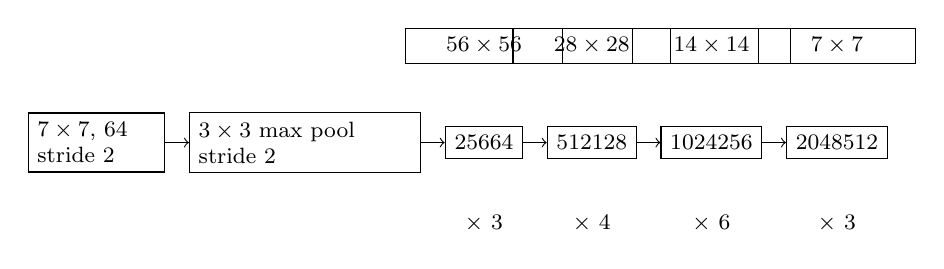
\begin{tikzpicture}[font=\footnotesize, node distance=0.3cm]
        {[start chain]
           \node[on chain,draw,text width=1.5cm] (conv1) {$7\times7$, 64\newline stride 2};
           \node[on chain,draw,join=by {->},text width=2.7cm] (pool) {$3\times3$ max pool\newline  stride 2};

           \node[on chain,draw,join=by {->}] (RB1) {\resblock{256}{64}};
           \node[below=0.8cm] at (RB1) {$\times$ 3};
           \node[above=1cm,draw,minimum width=2cm] at (RB1) {$56\times56$};

           \node[on chain,draw,join=by {->}] (RB2) {\resblock{512}{128}};
           \node[below=0.8cm] at (RB2) {$\times$ 4};
           \node[above=1cm,draw,minimum width=2cm] at (RB2) {$28\times28$};

           \node[on chain,draw,join=by {->}] (RB3) {\resblock{1024}{256}};
           \node[below=0.8cm] at (RB3) {$\times$ 6};
           \node[above=1cm,draw,minimum width=2cm] at (RB3) {$14\times14$};

           \node[on chain,draw,join=by {->}] (RB4) {\resblock{2048}{512}};
           \node[below=0.8cm] at (RB4) {$\times$ 3};
           \node[above=1cm,draw,minimum width=2cm] at (RB4) {$7\times7$};
        }
    \end{tikzpicture}
    \caption{Each bottleneck block has three \gls{conv} layers with their kernel sizes and channel count denoted in the graph. Beneath each block is the recurrence written and above are the output sizes for these blocks.
 }
    \label{fig:resnet50}
\end{figure}

For this work we use the 50-layered \gls{resnet} as described in the original paper. Its architecture is shown in \figreft{fig:resnet50}. At first stand a \gls{conv} layer with a big kernel size and stride 2 followed by a max pool thus reducing directly reducing the spatial size to a quarter. Then we build four chains of residual blocks each at a constant input size. Between the each chain we downscale by using a stride of 2 and in return double the channels. The last chain outputs $7 \times 7$ responses and with the average pooling layer we get to the singular score over the channels which are classified using the the final \gls{fc} layer.\\
This \gls{resnet} does not contain any dropout layers or different separate regularization elements. The original authors argue that the thin deep structure of this design does inherently regularize.


\clearpage
\section{Evaluation}
\label{sec:concepts:eval}
The result of this work is a binary object detector. Therefore a test run of the detector will result in a set of $n$ boxes $B_p$ that the method predicts as positive (object of the class the classifier was trained on) with probabilities $p_p \subset \mathbb{R}^n$. For the test set of images we know the actual ground truth boxes $B_g$ of this class. With some defined condition we mark the predicted boxes $B_p$ as true positive or false negative. The boxes from $B_g$ that were not predicted as positives by the detector are false negatives.

\subsubsection{Precision and Recall}
One way to evaluate a binary detector to plot the precision recall curves. Precision is defined as the proportion of the predicted positives that are actual positives:
\begin{equation}
    \textit{precision} = \frac{|B_p \cap B_g|}{|B_g|}
\end{equation}
Therefore a detector which does not predict any positives would have perfect precision even though it is obviously bad. The counteracting measure to use is the recall. Recall or also called \gls{tpr} states the proportion of all ground truth positives that are predicted positives:
\begin{equation}
    \textit{recall} = \textit{tpr} = \frac{|B_p \cap B_g|}{|B_p|}
\end{equation}
Here a detector that predicts only positives will receive perfect recall and as such we want a model with high precision and high recall.

Our detector returns probability scores for each positive predicted box and therefore we have to select an cut-off value for accepting positives. Now we can analyze how precision and recall change will we change this threshold. This transition is plotted in the precision-recall curve in which we plot precision against recall over the changing discrimination value.

\subsubsection{\gls{roc}}
Another often employed evaluation method are \gls{roc} curves and their \gls{auc}. For the \gls{roc} we pose the \gls{tpr} which tells how many of the positives we detected as positives against the \gls{fpr} which tells how many of the negatives were predicted as false positives. \gls{tpr} tells the probability that we hit a positive and \gls{fpr} tells the probability of an false alarm.

Plotting \gls{tpr} against \gls{fpr} over the changing discrimination threshold the same way as the precision-recall curve returns the \gls{roc} curve. The perfect detector would have a \gls{tpr} of 1 and a \gls{fpr} of 0 therefore we want a detector approaching this point of perfect classification. The \gls{roc} space reaches from 0 to 1 over both axes. A randomly guessing detector maps to the diagonal in this plot which as such is the discriminator between good and bad models.

To even summarize this metric more we calculate and report the \gls{auc} values for the different models. As the name states the \gls{auc} is the area under the \gls{roc} curve with values in $[0, 1]$. Because the random classifier returns the diagonal inside the \gls{roc} space the \gls{auc} value can be interpreted as the probability that a detector will score a positive ground truth sample higher than a negative one. With \gls{auc} of 1 that would be perfect with 0.5 it would be random. We calculate the \gls{auc} with the trapezoidal rule applied to the \gls{roc} curve.
       % INCLUDE: concepts
% % !TEX root = ../thesis.tex
%
\chapter{Conclusion}
\label{sec:conclusion}
This thesis presents a image retrieval system employing a \acrlong{fcn} for efficient object detection. For this the underlying \gls{resnet} is quickly and without the objective of convergence fine-tuned with a set of heavily augmented versions of the query image. The linear classifier is converted to a convolutional operator to perform sparse class probability prediction on images of any size. Using these probability maps we predict the existence of the query object inside larger images and yield those patches.

Although the method proved successful in finding similar objects with only few or only one query image to train from, we the presented method ha  
     % INCLUDE: conclusion

% --------------------------
% Back matter
% --------------------------
\appendix\cleardoublepage
% % !TEX root = ../thesis.tex
%
\chapter{Appendix}
\label{sec:appendix}

\section{\textsc{Pascal}-Part class-part combinations}
\label{sec:appendix:combos}
\begin{table}[h]
	\label{tab:combos}
	\centering
	\begin{tabulary}{\textwidth}{LLL}
		Tag & Classes & Parts \\ \hline
		\code{aeroplane\_lwing\_rwing} & Plane & Left wing, right wing \\ %\hline
		\code{aeroplane\_stern} & Plane & Stern (Rudder) \\ %\hline
		\code{bicycle\_bwheel\_fwheel} & Bicycle & Back wheel, front wheel\\ %\hline
		\code{bird\_beak} & Bird & Beak \\ %\hline
		\code{bird\_head} & Bird & Head \\ %\hline
		\code{bird\_lwing\_rwing} & Bird & Left wing, right wing\\ %\hline
		\code{bird\_tail} & Bird & Tail \\ %\hline
		\code{bottle\_body} & Bottle & Body \\ %\hline
		\code{bus\_car\_bliplate\_fliplate} & Bus, Car & Front and back license plate \\ %\hline
		\code{car\_door} & Car & door \\ %\hline
		\code{cow\_sheep\_lhorn\_rhorn} & Cow, Sheep & Left horn, right horn \\ %\hline
		\code{motorbike\_bwheel\_fwheel} & Motorbike & Front wheel, back wheel \\ %\hline
		\code{person\_hair} & Person & Hair \\ %\hline
		\code{person\_head} & Person & Head \\ %\hline
		\code{person\_lear\_rear} & Person & Left ear, right ear \\ %\hline
		\code{person\_lfoot\_rfoot} & Person & Left foot, right foot \\ %\hline
		\code{person\_lhand\_rhand} & Person & Left hand, right hand \\ %\hline
		\code{person\_neck} & Person & Neck \\ %\hline
		\code{person\_torso} & Person & Torso \\ %\hline
		\code{pottedplant\_plant} & Potted plant & Plant \\ %\hline
		\code{train\_coach} & Train & Coach (normal carriage) \\ %\hline
		\code{train\_head} & Train & Head (motor coach) \\ %\hline
		\code{train\_hfrontside} & Train & Head front side
	\end{tabulary}
\end{table}

\clearpage
\section{\textsc{Pascal}-Part test results}
\label{sec:appendix:pr_roc}
\begin{longtabu} to \textwidth {XX}
    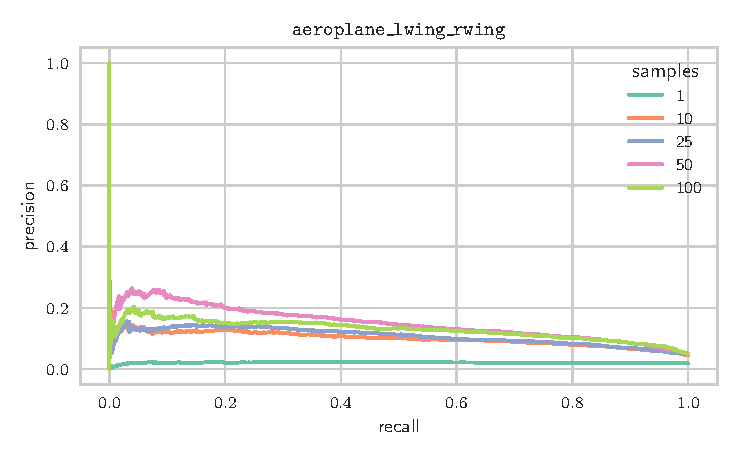
\includegraphics[width=0.47\textwidth]{figures/build/aeroplane_lwing_rwing_precs_recs.pdf} &
    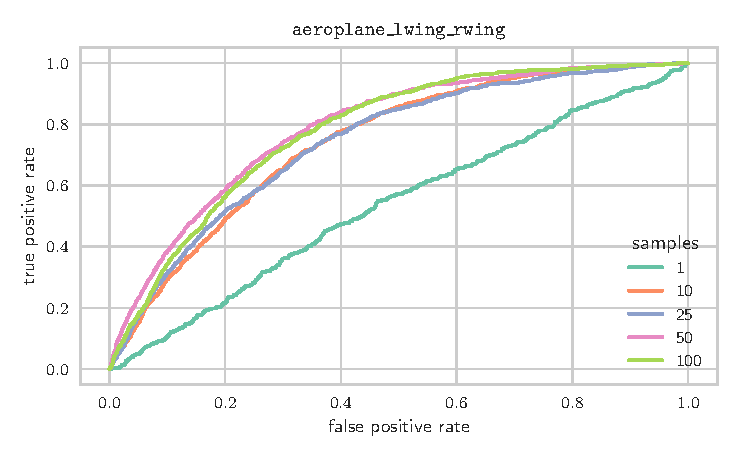
\includegraphics[width=0.47\textwidth]{figures/build/aeroplane_lwing_rwing_roc.pdf} \\
    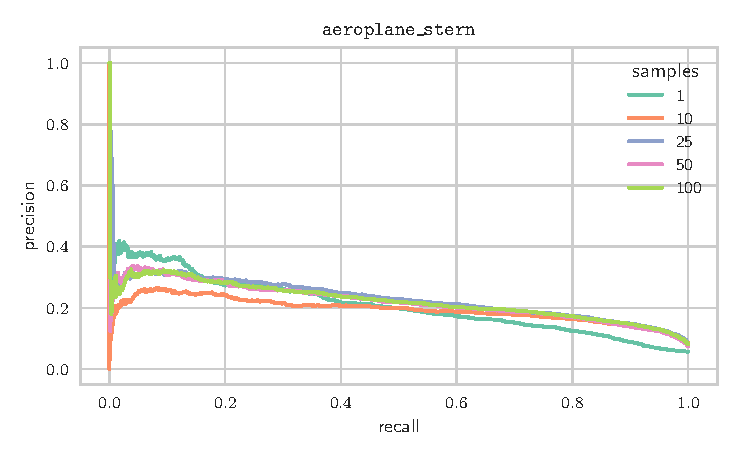
\includegraphics[width=0.47\textwidth]{figures/build/aeroplane_stern_precs_recs.pdf} &
    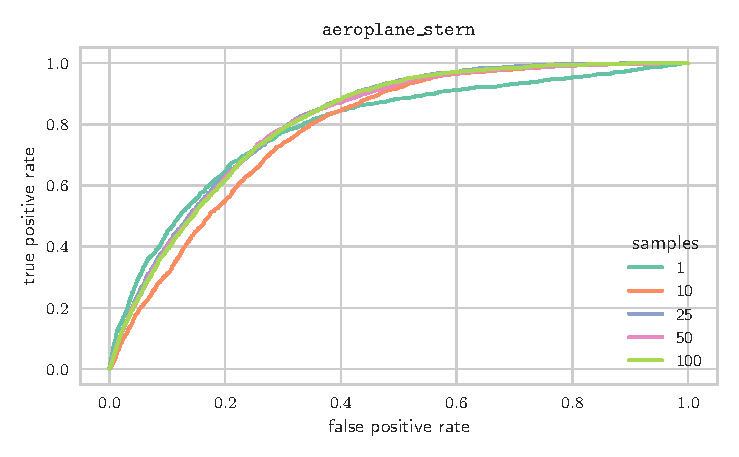
\includegraphics[width=0.47\textwidth]{figures/build/aeroplane_stern_roc.pdf} \\
    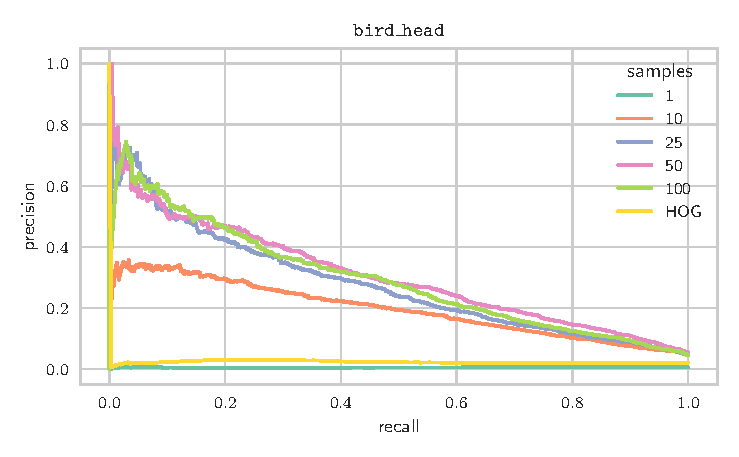
\includegraphics[width=0.47\textwidth]{figures/build/bird_head_precs_recs.pdf} &
    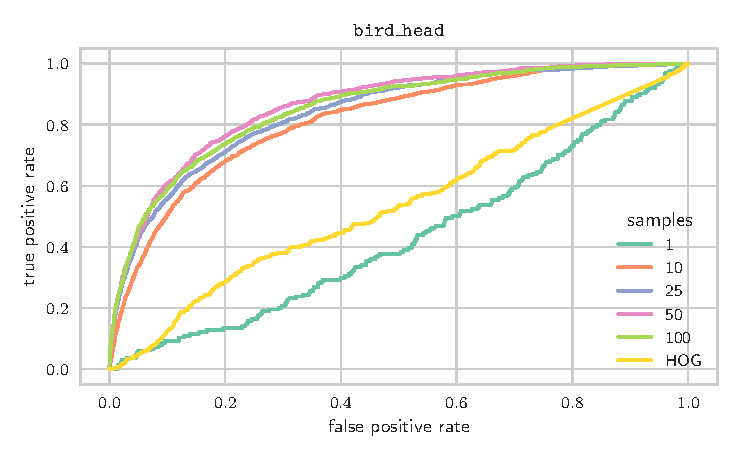
\includegraphics[width=0.47\textwidth]{figures/build/bird_head_roc.pdf} \\
    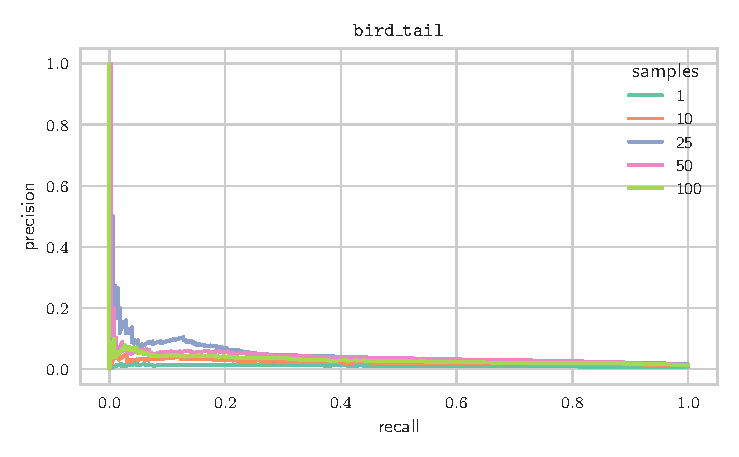
\includegraphics[width=0.47\textwidth]{figures/build/bird_tail_precs_recs.pdf} &
    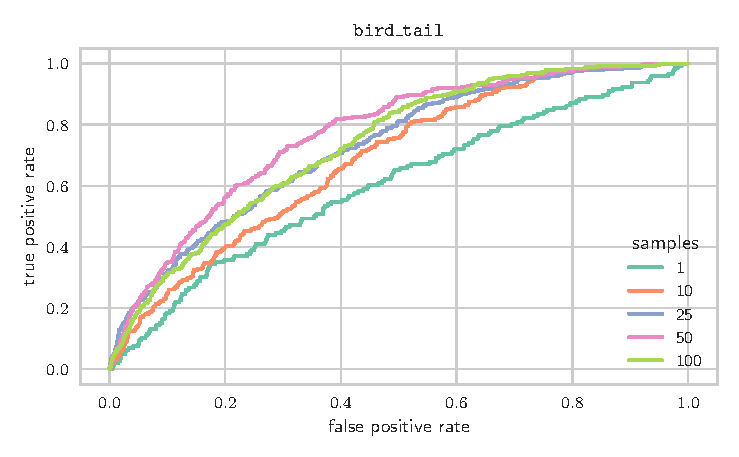
\includegraphics[width=0.47\textwidth]{figures/build/bird_tail_roc.pdf} \\
    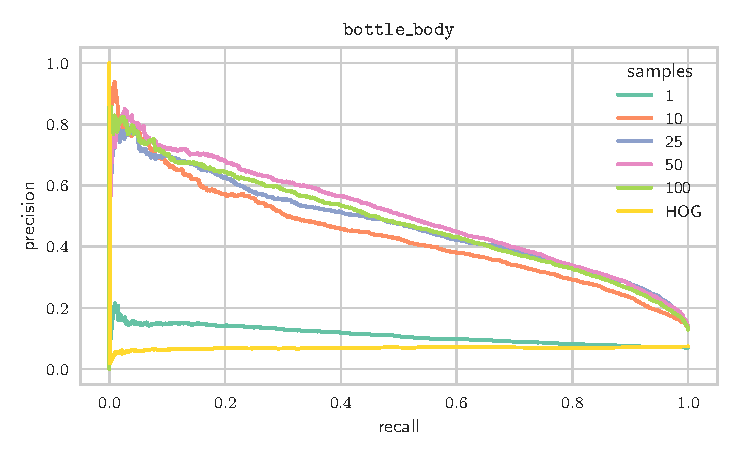
\includegraphics[width=0.47\textwidth]{figures/build/bottle_body_precs_recs.pdf} &
    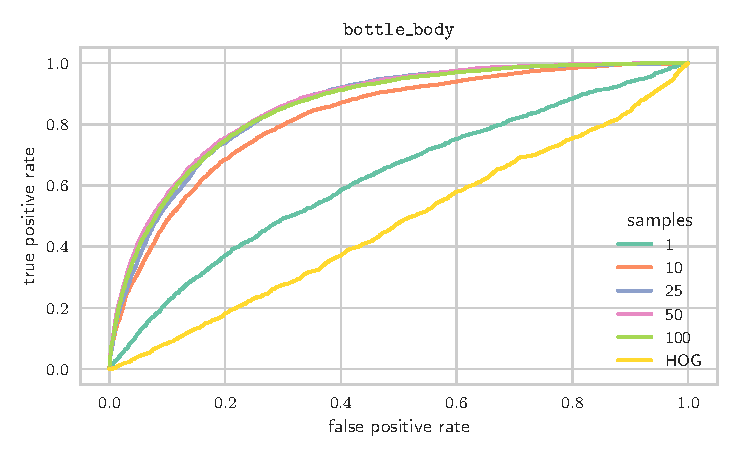
\includegraphics[width=0.47\textwidth]{figures/build/bottle_body_roc.pdf} \\
    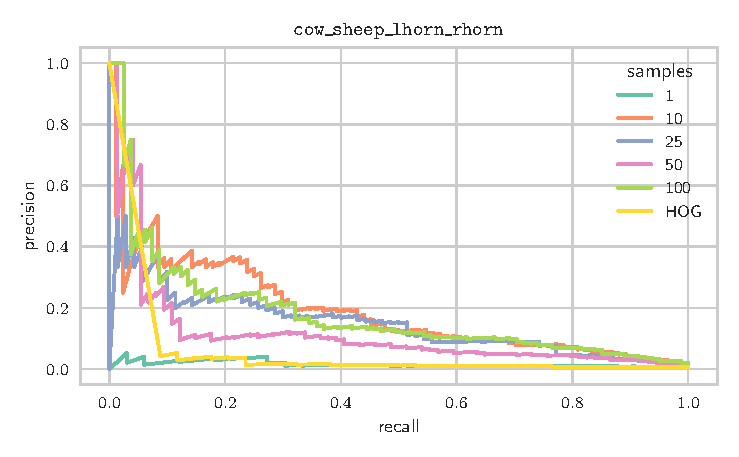
\includegraphics[width=0.47\textwidth]{figures/build/cow_sheep_lhorn_rhorn_precs_recs.pdf} &
    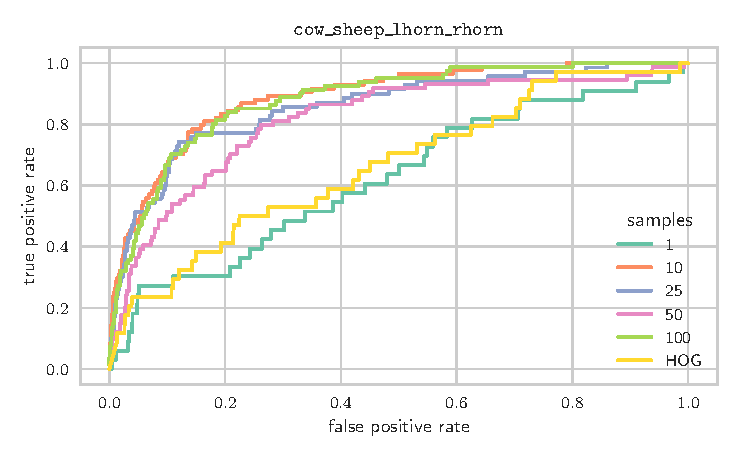
\includegraphics[width=0.47\textwidth]{figures/build/cow_sheep_lhorn_rhorn_roc.pdf} \\
    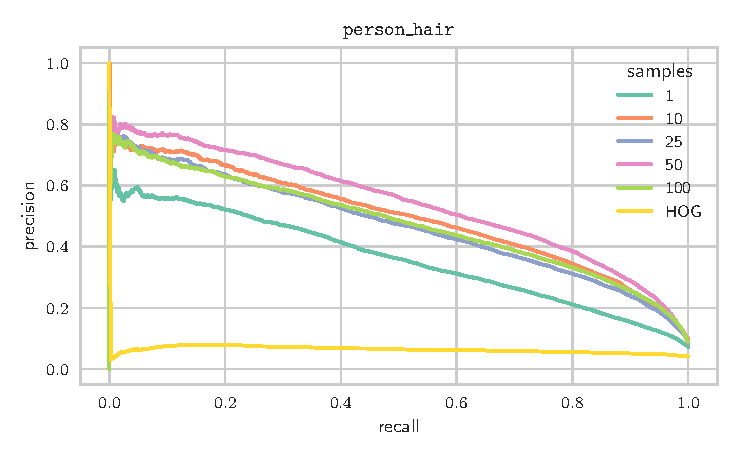
\includegraphics[width=0.47\textwidth]{figures/build/person_hair_precs_recs.pdf} &
    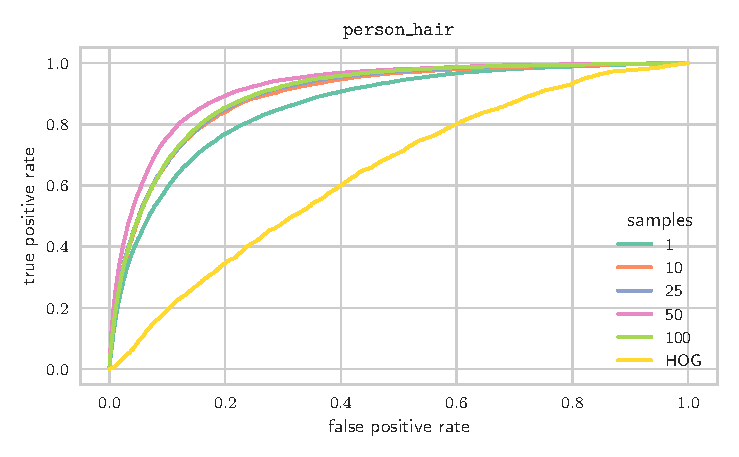
\includegraphics[width=0.47\textwidth]{figures/build/person_hair_roc.pdf} \\
    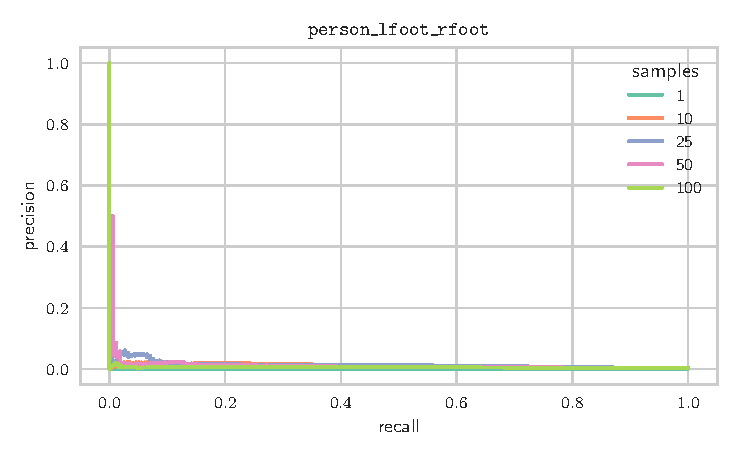
\includegraphics[width=0.47\textwidth]{figures/build/person_lfoot_rfoot_precs_recs.pdf} &
    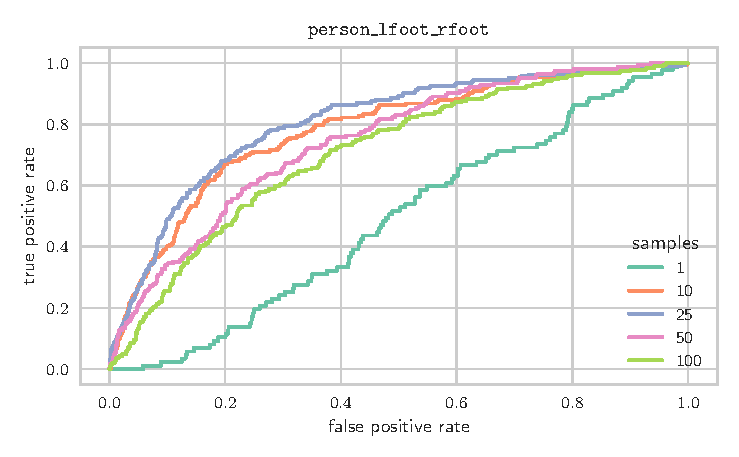
\includegraphics[width=0.47\textwidth]{figures/build/person_lfoot_rfoot_roc.pdf} \\
    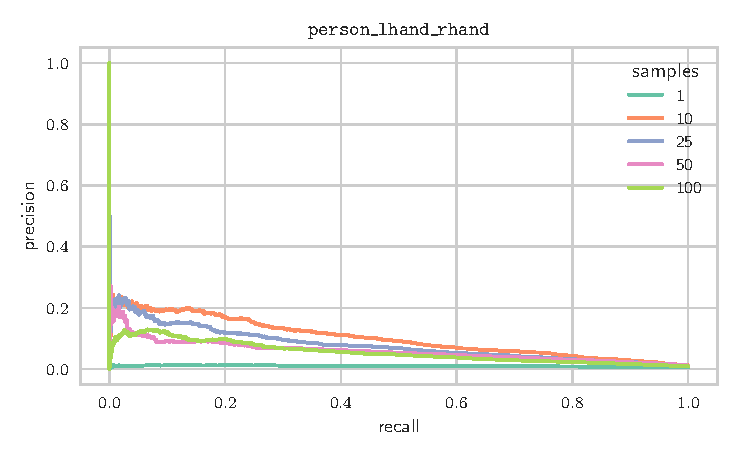
\includegraphics[width=0.47\textwidth]{figures/build/person_lhand_rhand_precs_recs.pdf} &
    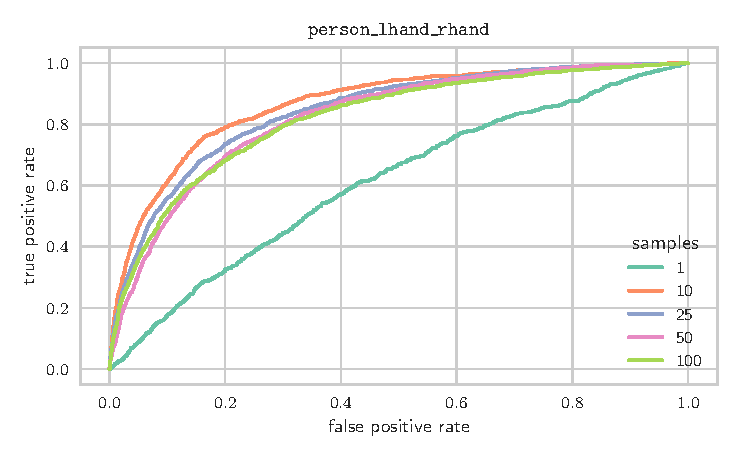
\includegraphics[width=0.47\textwidth]{figures/build/person_lhand_rhand_roc.pdf} \\
    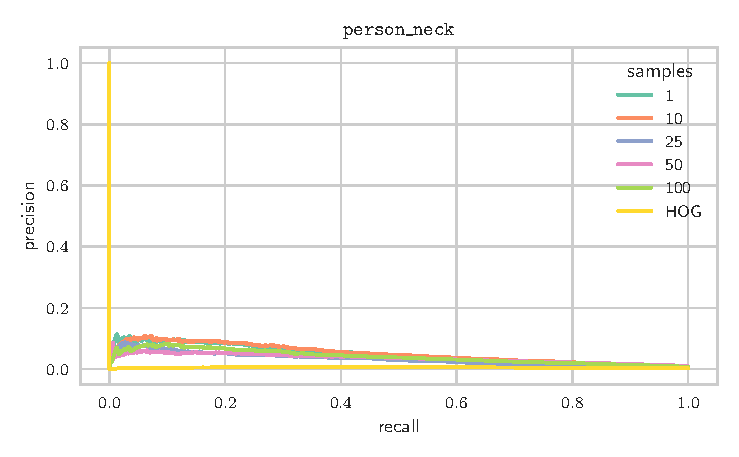
\includegraphics[width=0.47\textwidth]{figures/build/person_neck_precs_recs.pdf} &
    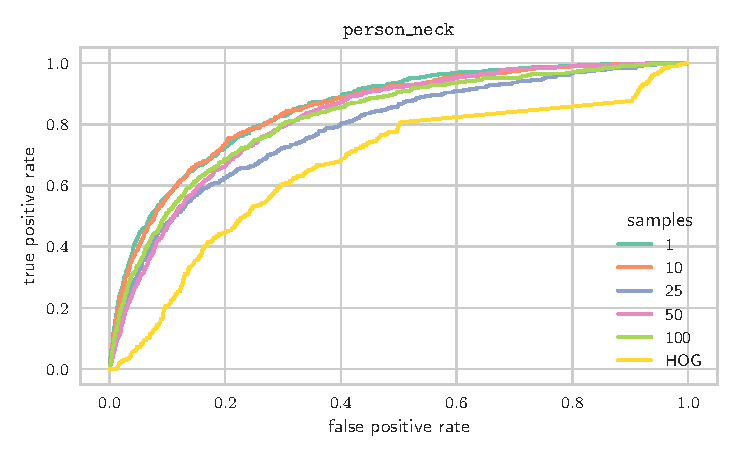
\includegraphics[width=0.47\textwidth]{figures/build/person_neck_roc.pdf} \\
    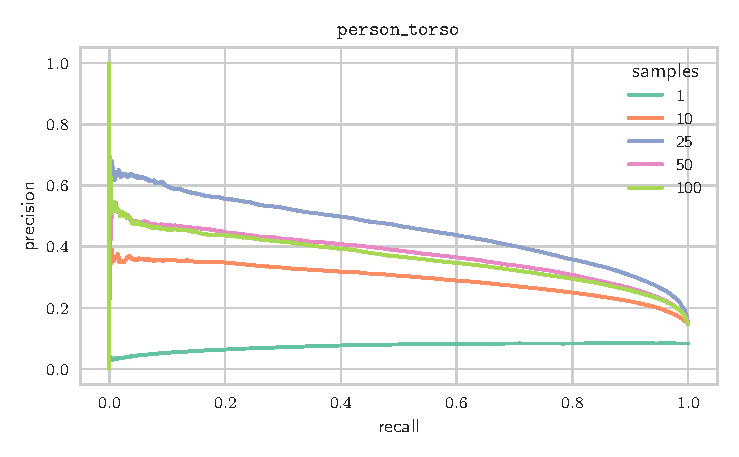
\includegraphics[width=0.47\textwidth]{figures/build/person_torso_precs_recs.pdf} &
    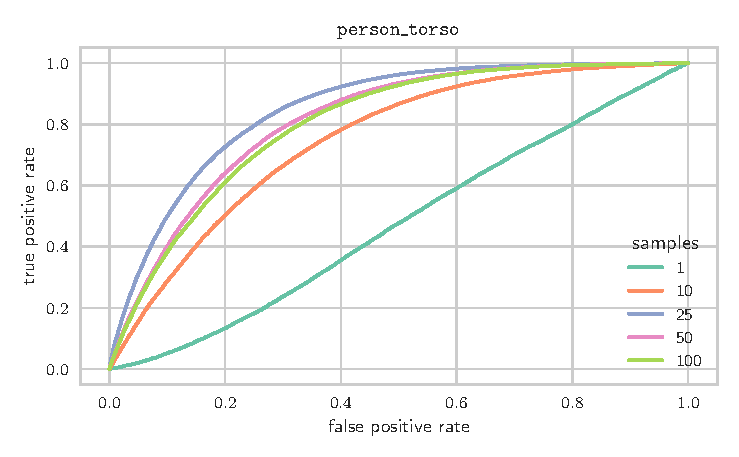
\includegraphics[width=0.47\textwidth]{figures/build/person_torso_roc.pdf} \\
    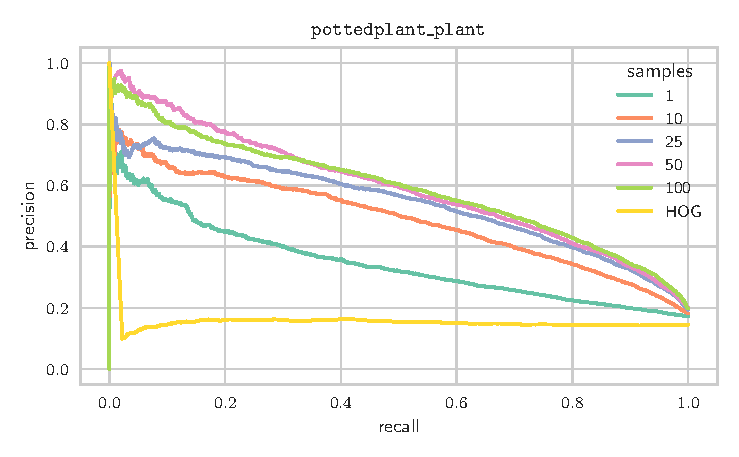
\includegraphics[width=0.47\textwidth]{figures/build/pottedplant_plant_precs_recs.pdf} &
    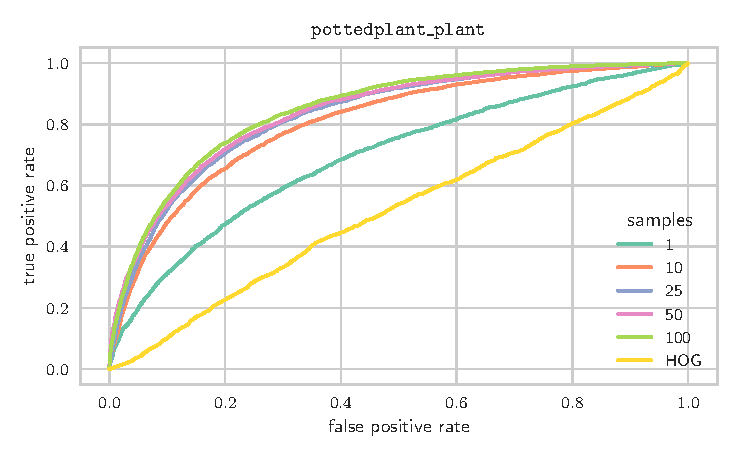
\includegraphics[width=0.47\textwidth]{figures/build/pottedplant_plant_roc.pdf} \\
    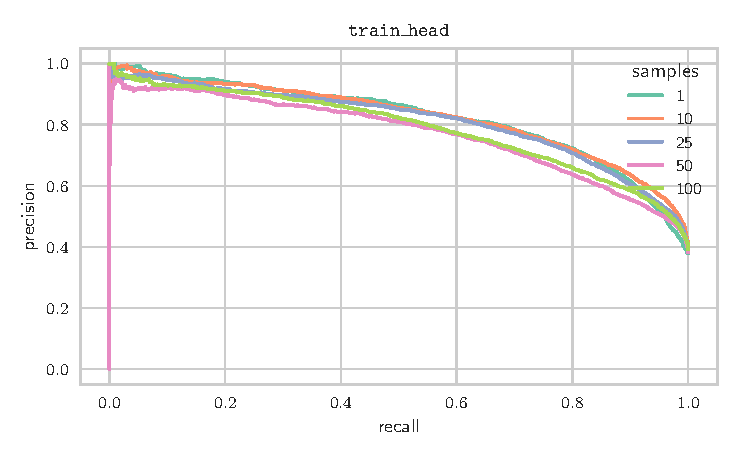
\includegraphics[width=0.47\textwidth]{figures/build/train_head_precs_recs.pdf} &
    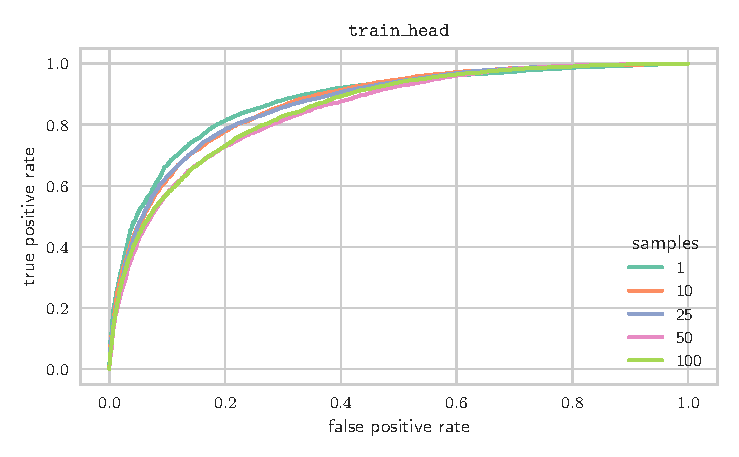
\includegraphics[width=0.47\textwidth]{figures/build/train_head_roc.pdf}
	\label{tab:combos}
\end{longtabu}
       % INCLUDE: appendix
%
{%
\printglossaries
\cleardoublepage

\setstretch{1.1}
\renewcommand{\bibfont}{\normalfont\small}
\setlength{\biblabelsep}{0pt}
\setlength{\bibitemsep}{0.5\baselineskip plus 0.5\baselineskip}
\printbibliography[nottype=online]
\printbibliography[heading=subbibliography,title={Webpages},type=online,prefixnumbers={@}]
}
\cleardoublepage

\listoffigures
\cleardoublepage

\listoftables
\cleardoublepage

% \input{chapters/colophon}
\cleardoublepage

% !TEX root = ../thesis.tex
%
%************************************************
% Declaration
%************************************************
\pdfbookmark[0]{Erklärung}{Erklärung}
\chapter*{Erklärung}
\label{sec:declaration}
\thispagestyle{empty}

Ich versichere, dass ich diese Arbeit selbstständig verfasst und keine anderen als die angegebenen Quellen und Hilfsmittel benutzt habe.
\bigskip

\noindent\textit{\thesisUniversityCity, \thesisDate}

\smallskip

\begin{flushright}
	\begin{minipage}{5cm}
		\rule{\textwidth}{1pt}
		\centering\thesisName
	\end{minipage}
\end{flushright}

%*****************************************
%*****************************************

\clearpage
\newpage
\mbox{}

% **************************************************
% End of Document CONTENT
% **************************************************
\end{document}
